\chapter{Конструкторская часть}

В данном разделе будут приведены схемы конвейерной и линейной реализаций алгоритма поиска подстроки в строке.

\section{Разработка алгоритмов}

На рис. \ref{fig:linear_processing} -- \ref{fig:stages} приведены схемы линейной и конвейерной реализаций алгоритма поиска подстроки в строке, схема трёх лент для конвейерной обработки строки, а также схемы реализаций этапов обработки строки.


\begin{figure}[h]
	\centering
	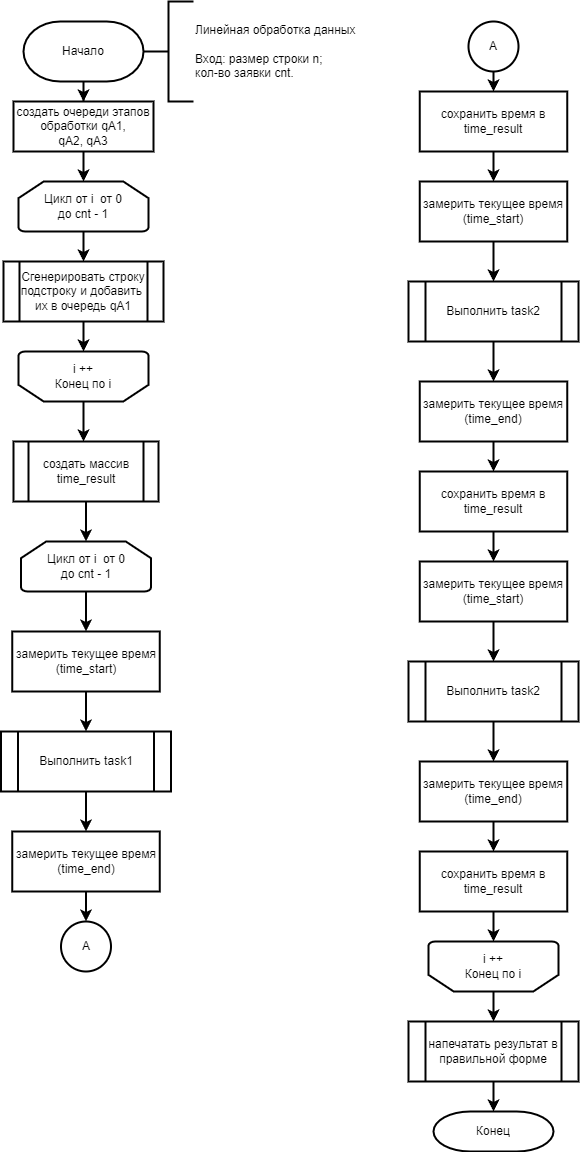
\includegraphics[scale=0.55]{img/linear_processing.png}
	\caption{Схема алгоритма линейной обработки строки}
	\label{fig:linear_processing}
\end{figure}

\clearpage

\begin{figure}[h]
	\centering
	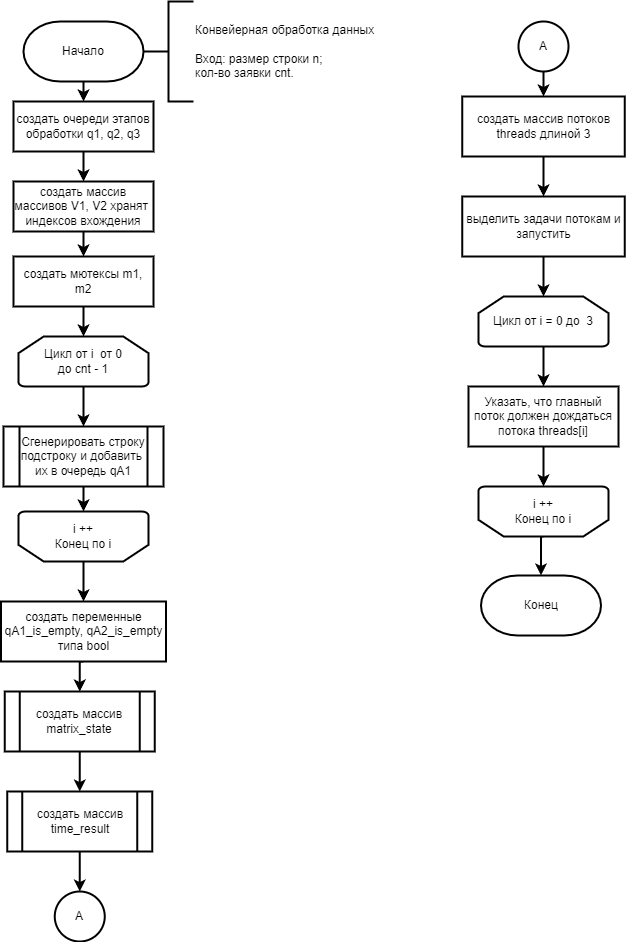
\includegraphics[scale=0.6]{img/parallel_processing.png}
	\caption{Схема алгоритма конвейерной обработки строки}
	\label{fig:parallel_processing}
\end{figure}

\clearpage

\begin{figure}[h]
	\centering
	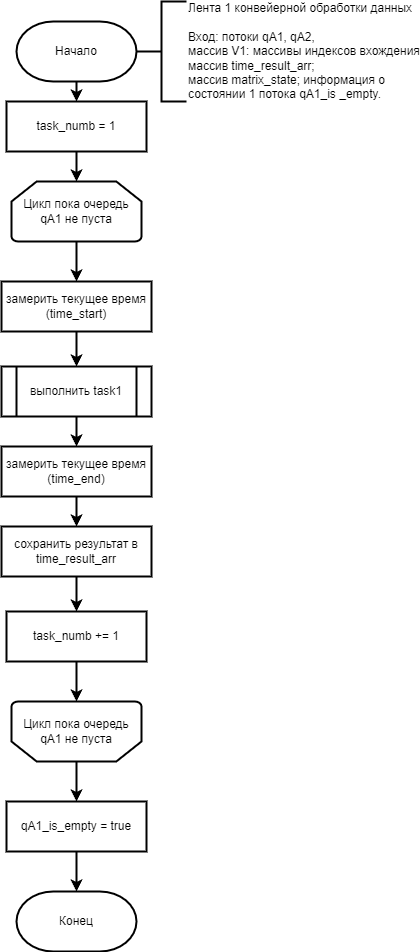
\includegraphics[scale=0.6]{img/parallel_stage_1.png}
	\caption{Схема 1-ой ленты конвейерной обработки строки}
	\label{fig:parallel_stage_1}
\end{figure} 

\clearpage

\begin{figure}[h]
	\centering
	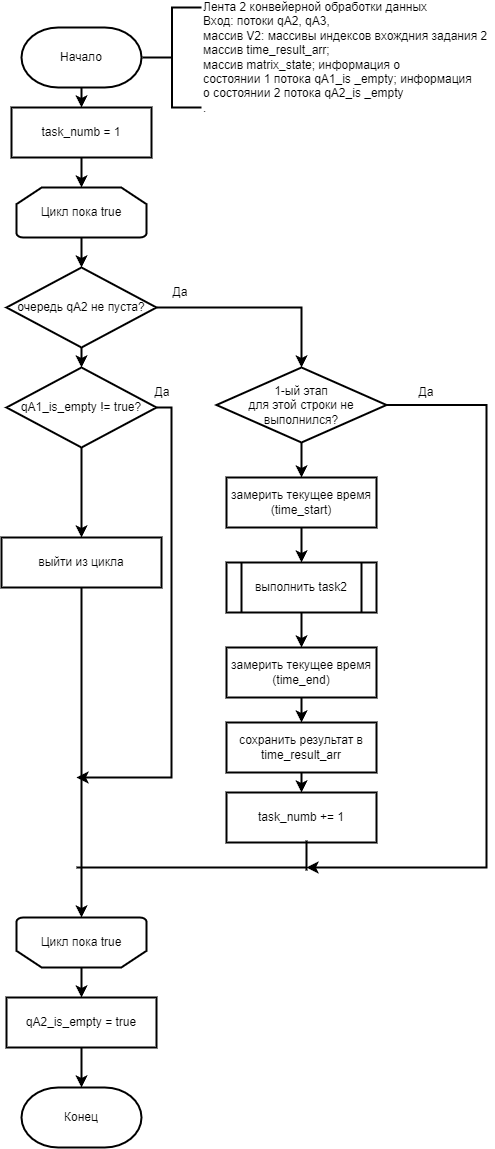
\includegraphics[scale=0.5]{img/parallel_stage_2.png}
	\caption{Схема 2-ой ленты конвейерной обработки строки}
	\label{fig:parallel_stage_2}
\end{figure} 

\clearpage

\begin{figure}[h]
	\centering
	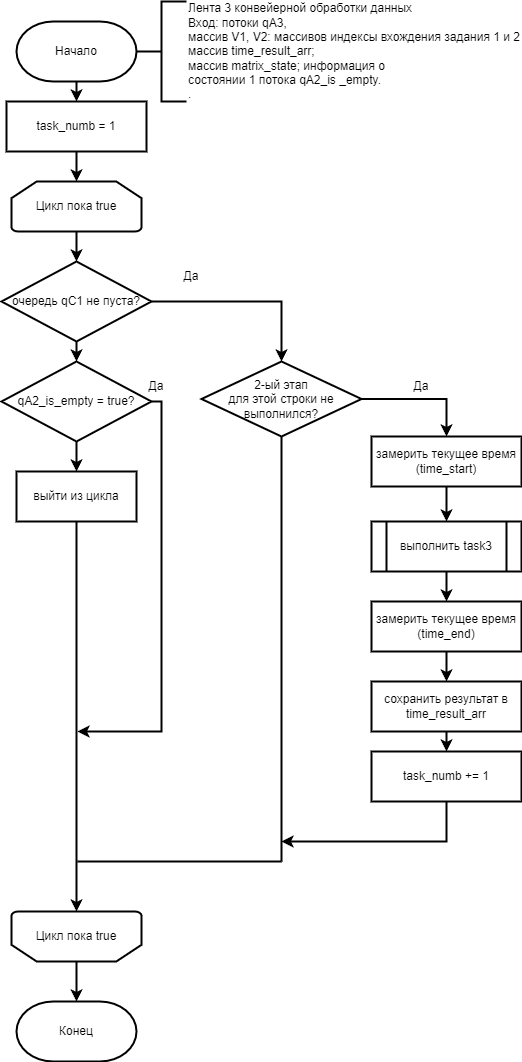
\includegraphics[scale=0.5]{img/parallel_stage_3.png}
	\caption{Схема 3-ей ленты конвейерной обработки строки}
	\label{fig:parallel_stage_3}
\end{figure} 

\clearpage

\begin{figure}[h]
	\centering
	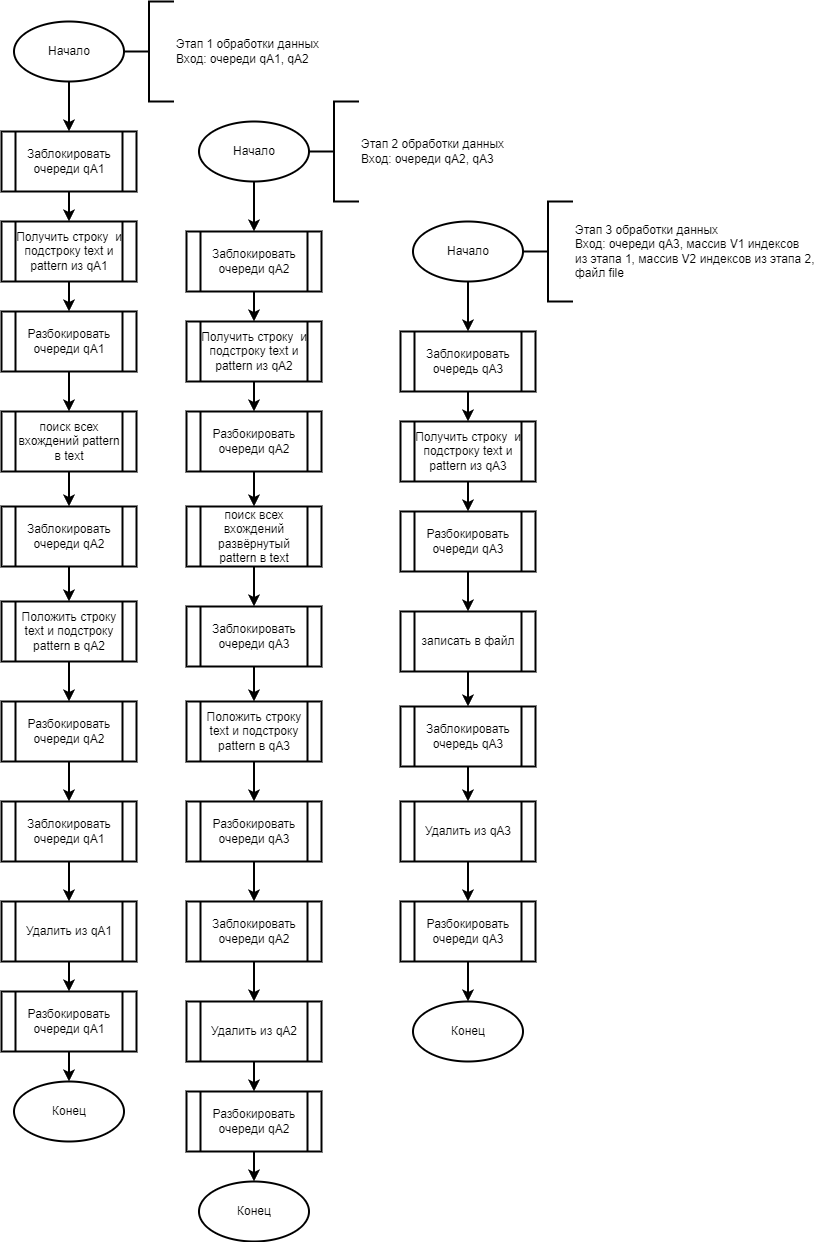
\includegraphics[scale=0.5]{img/stages.png}
	\caption{Схема реализаций этапов обработки строки}
	\label{fig:stages}
\end{figure} 

\clearpage

\section{Требования к программному обеспечению}

Входные данные задается размер строки и количество строк, которое должно быть больше 0. 

Выходные данные --- табличка с размерами строки, количествами строк, номерами этапов (лент) её обработки, временем начала обработки текущей строки на текущей ленте, временем окончания обработки текущей строки на текущей ленте.


\section{Классы эквивалентности}

Выделенные классы эквивалентности для тестирования:

\begin{itemize}[label=---]
	\item размер строки <= 0;
	\item размер строки не является целым числом;
	\item количество заявок <= 0;
	\item номер команды < 0 или > 3;
	\item номер команды не является целым числом;
\end{itemize}



\section*{Вывод}

В данном разделе на основе теоретических данных были построены схемы требуемых методов обработки строки (конвейерного и линейного), приведены требования к программному обеспечению и выделены классы эквивалентности для тестирования.

\clearpage